\documentclass[tikz,convert={outfile=\jobname.svg,command=\unexpanded{pdf2svg \infile\space\outfile}}]{standalone}

\usepackage{amsmath}

\usepackage[outline]{contour}
\contourlength{0.14em} % default is 0.05em, values >0.14em lead to clipped arrows


\usepackage{color}
\definecolor{figurehighlight1}{RGB}{190, 0, 0}
\definecolor{figurehighlight2}{RGB}{0, 0, 190}
\definecolor{anthrazit}{RGB}{ 50, 50, 50}
\definecolor{mittelblau}{RGB}{0,  65,  145}
\definecolor{hellblau}{RGB}{  0,  190, 255}
\definecolor{dunkelrot}{RGB}{  190,  0, 0}
\definecolor{kommentare}{RGB}{0, 99, 0}
\definecolor{gelb}{RGB}{222, 173, 0}
\definecolor{linkcolor}{rgb}{0,0,0.5}


\usetikzlibrary{fit,positioning,arrows.meta,decorations.pathreplacing,calc, backgrounds,snakes,arrows,decorations.markings,shapes.misc}

\tikzset{% basics
  every node/.style={font=\scriptsize,align=center},
  annex_lifeline/.style={draw=black!30},
  annex_lifeline_dotted/.style={draw=anthrazit,dotted},
  annex_matrix_node/.style={},
  annex_matrix_dummy_height/.style={},
  % default style used below
  line/.style={draw=yellow!50!green},
  seperatorline/.style={draw=hellblau},
  reqrespline/.style={draw=mittelblau, line width=0.25mm},
  websocketline/.style={draw=gelb, line width=0.2mm},
  % groups
  annex_group_box/.style={draw=black!15,fill=black!4,dashed,rounded corners=1ex},
  annex_group_title_placeholder/.style={},
  annex_condensed_box/.style={draw=blue,rounded corners=1ex,inner sep=0.3ex},
  annex_multistep_caption_text/.style={blue},%font=\sffamily\tiny\color{teal}},
  % start/end parties
%  annex_start_party_box/.style={fill=white,draw,rounded corners=0.3ex,align=center,anchor=center,text height=5pt,text depth=0ex,minimum height=0em,inner sep=1.5mm},
 annex_start_party_box/.style={fill=white,draw,rounded corners=0.3ex,align=center,anchor=center,inner sep=1mm},
  annex_end_party_box/.style={annex_start_party_box,scale=0.8},
  % individual steps
  annex_arrow_text/.style={yshift=1pt},
  annex_message/.style={fill=white,-Latex,reqrespline},
  annex_http_request/.style={fill=white,-Latex,reqrespline},
  annex_http_response/.style={-Latex[open],reqrespline,align=center},
  annex_websocket/.style={-Latex,websocketline},
  annex_action/.style={fill=white,inner sep=0ex,minimum height=1em,align=center},
  annex_open_window/.style={->,line,dashed},
  annex_script_action_box/.style={annex_action,anchor=center},
  annex_script_action_arrow/.style={-Latex[open],reqrespline},
  annex_script_action_arrow_reversed/.style={<-,line},
  annex_open_window_start_party_box/.style={annex_start_party_box},
  annex_open_window_start_party_arrow/.style={->,line,dashed},
  annex_separator/.style={seperatorline,dashed},
  server/.style={draw=anthrazit,fill=anthrazit,text=white},
  browser/.style={},
  attacker/.style={draw=dunkelrot,fill=dunkelrot,text=white},
  annex_comment_text/.style={font=\small},
  annex_vertical_space/.style={},
  msg_type/.style={align=left,xshift=1pt,font=\scriptsize\scshape,rounded corners=1pt,inner sep=2pt,text depth=1pt,text height=4pt,gray},
  annex_note/.style={align=left},
  annex_debug/.style={opacity=0},
}


% Uppercase roman numbering
\newcounter{bigprotophase}[figure]
\renewcommand{\thebigprotophase}{\Roman{bigprotophase}}
\def\bigprotophase#1{%
  \begin{tikzpicture}
    \node[rounded corners,fill=OliveGreen]{%
      \parbox{1.4em}{%
        \color{white}\centering%
        \textbf{%
          \refstepcounter{bigprotophase}%
          \thebigprotophase%
          \label{bigprotophase:#1}%
        }%
      }%
    };%
  \end{tikzpicture}%
}

\def\refbigprotophase#1{%
  \resizebox{!}{0.6\baselineskip}{%
    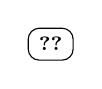
\begin{tikzpicture}[baseline={([yshift=-1.5pt]O.base)}]
      \node (O) [draw,rounded corners]{\parbox{1.2em}{\centering\ref{bigprotophase:#1}}};
    \end{tikzpicture}%
  }%
}


% Lowercase roman numbering
\newcounter{protophase}[figure]
\renewcommand{\theprotophase}{\roman{protophase}}
\def\protophase#1{%
  \begin{tikzpicture}
    \node [rounded corners,fill=OliveGreen]{%
      \parbox{1.2em}{%
        \color{white}\centering%
        \textbf{%
          \refstepcounter{protophase}%
          \theprotophase%
          \label{protophase:#1}%
        }%
      }%
    };%
  \end{tikzpicture}%
}

\def\refprotophase#1{%
  \resizebox{!}{0.6\baselineskip}{%
    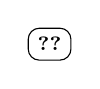
\begin{tikzpicture}[baseline={([yshift=-1.5pt]O.base)}]
      \node (O) [draw,rounded corners]{\parbox{1.1em}{\centering\ref{protophase:#1}}};
    \end{tikzpicture}%
  }%
}


% Regular numbering
\newcounter{protostep}[figure]
\def\protostep#1{%
  \resizebox{!}{0.8\baselineskip}{%
    \begin{tikzpicture}[baseline={([yshift=-0.5pt]O.base)}]
      \node (O) [sharp corners,fill=blue,inner sep=1ex]{%
        \color{white}%
        \textbf{%
          \refstepcounter{protostep}%
          \theprotostep%
          \label{protostep:#1}%
        }%
      };
    \end{tikzpicture}%
  }%
}

\def\refprotostep#1{%
  \resizebox{!}{0.6\baselineskip}{%
    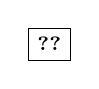
\begin{tikzpicture}[baseline={([yshift=-1.5pt]O.base)}]
      \node (O) [draw,sharp corners]{\ref{protostep:#1}};
    \end{tikzpicture}%
  }%
}

% alphabetical "numbering"
\newcounter{attackstep}[figure]
\renewcommand{\theattackstep}{\alph{attackstep}}
\def\attackstep#1{%
  \resizebox{!}{0.8\baselineskip}{%
    \begin{tikzpicture}[baseline={([yshift=-0.5pt]O.base)}]
      \node (O) [draw,sharp corners]{%
        \textbf{%
          \refstepcounter{attackstep}%
          \theattackstep%
          \label{attackstep:#1}%
        }%
      };
    \end{tikzpicture}%
  }%
}

\def\refattackstep#1{%
  \resizebox{!}{0.6\baselineskip}{%
    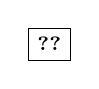
\begin{tikzpicture}[baseline={([yshift=-1.5pt]O.base)}]
      \node (O) [draw,sharp corners]{\ref{attackstep:#1}};
    \end{tikzpicture}%
  }%
}

%%%%%%%%%%%%%%%%%%%%%%%%%%%
% END of annexlang macros %
%%%%%%%%%%%%%%%%%%%%%%%%%%%

\begin{document}

        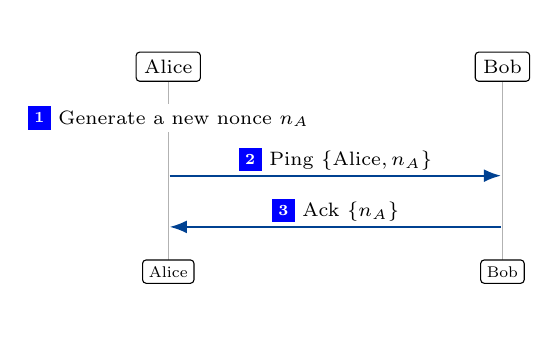
\begin{tikzpicture}[]
        \pgfdeclarelayer{arrows}
        \pgfdeclarelayer{groups}
        \pgfdeclarelayer{markers}
        \pgfsetlayers{groups,arrows,main,markers}
        
        % MATRIX
        \matrix [column sep={0.35\linewidth,between origins}, row sep=0.3ex]
        {
        \node[annex_matrix_node,inner sep=0,outer sep=0](pos-0-0){}; &\node[annex_matrix_node,inner sep=0,outer sep=0](pos-1-0){};\node[annex_matrix_dummy_height,minimum height=5ex,anchor=center]{};\node[annex_matrix_dummy_height,minimum height=5ex,anchor=center]{};\\
\node[annex_matrix_node,inner sep=0,outer sep=0](pos-0-1){}; &\node[annex_matrix_node,inner sep=0,outer sep=0](pos-1-1){};\node[annex_matrix_dummy_height,minimum height=3ex,anchor=center]{};\\
\node[annex_matrix_node,inner sep=0,outer sep=0](pos-0-2){}; &\node[annex_matrix_node,inner sep=0,outer sep=0](pos-1-2){};\node[annex_matrix_dummy_height,minimum height=2ex+2ex,anchor=south,yshift=-1ex]{};\\
\node[annex_matrix_node,inner sep=0,outer sep=0](pos-0-3){}; &\node[annex_matrix_node,inner sep=0,outer sep=0](pos-1-3){};\node[annex_matrix_dummy_height,minimum height=2ex+2ex,anchor=south,yshift=-1ex]{};\\
\node[annex_matrix_node,inner sep=0,outer sep=0](pos-0-4){}; &\node[annex_matrix_node,inner sep=0,outer sep=0](pos-1-4){};\node[annex_matrix_dummy_height,minimum height=5ex,anchor=center]{};\node[annex_matrix_dummy_height,minimum height=5ex,anchor=center]{};\\
};

% MAIN LAYER

% drawing node of type Protocol in matrix line 0 with attributes: {'annexid': 'Protocol_1', 'parties': [<Party_2>, <Party_3>], 'steps': [<Parallel_4>, <Action_5>, <GenericMessage_6>, <GenericMessage_7>, <Parallel_8>], 'options': {'colsep': '0.35\\linewidth', 'rowsep': '0.3ex', 'enumerate': '\\setcounter{protostep}{%d}\\protostep{2msg-example:%s} ', 'styles': [], 'tex_intro': ''}, 'line': 0, 'length': 5, 'columns': [{'num': 0}, {'num': 1}], 'protocol': <Protocol_1>}


% drawing node of type Parallel in matrix line 0 with attributes: {'annexid': 'Parallel_4', 'steps': [<StartParty_9>, <StartParty_10>], 'line': 0, 'length': 1, 'protocol': <Protocol_1>}


% drawing node of type StartParty in matrix line 0 with attributes: {'annexid': 'StartParty_9', 'party': <Party_2>, 'line': 0, 'protocol': <Protocol_1>, 'node_name_counter': 1, '_affecting_nodes': ['StartParty_9_0'], 'node_name': 'StartParty_9_0', 'end': <EndParty_11>, 'lifeline_segments': [(0, 8, 'annex_lifeline')]}
\node[name=StartParty_9_0,annex_start_party_box,] at (pos-0-0) {Alice};

% drawing node of type StartParty in matrix line 0 with attributes: {'annexid': 'StartParty_10', 'party': <Party_3>, 'line': 0, 'protocol': <Protocol_1>, 'node_name_counter': 1, '_affecting_nodes': ['StartParty_10_0'], 'node_name': 'StartParty_10_0', 'end': <EndParty_12>, 'lifeline_segments': [(0, 8, 'annex_lifeline')]}
\node[name=StartParty_10_0,annex_start_party_box,] at (pos-1-0) {Bob};

% drawing node of type Action in matrix line 1 with attributes: {'annexid': 'Action_5', 'party': <Party_2>, 'id': 'gen-nonce', 'label': 'Generate a new nonce $n_A$', 'line': 1, 'protocol': <Protocol_1>, '_counter': 1, 'node_name_counter': 1, '_affecting_nodes': ['Action_5_0'], 'node_name': 'Action_5_0'}
\node[annex_action,name=Action_5_0,pin={[pin distance=-6pt,pin edge={draw=none},annex_debug]90:{gen-nonce} }] at (pos-0-1) {\setcounter{protostep}{0}\protostep{2msg-example:gen-nonce} \contour{white}{Generate a new nonce $n_A$}};

% drawing node of type GenericMessage in matrix line 2 with attributes: {'annexid': 'GenericMessage_6', 'src': <Party_2>, 'dest': <Party_3>, 'caption': 'Ping $\\{\\text{Alice}, n_A\\}$', 'id': 'online-msg1', 'line': 2, 'protocol': <Protocol_1>, '_counter': 2, 'text_above': 'Ping $\\{\\text{Alice}, n_A\\}$', 'text_below': '', '_affecting_nodes': ['pos-0-2', 'pos-1-2']}


% drawing node of type GenericMessage in matrix line 3 with attributes: {'annexid': 'GenericMessage_7', 'src': <Party_3>, 'dest': <Party_2>, 'caption': 'Ack $\\{n_A\\}$', 'line': 3, 'protocol': <Protocol_1>, '_counter': 3, 'text_above': 'Ack $\\{n_A\\}$', 'text_below': '', '_affecting_nodes': ['pos-1-3', 'pos-0-3']}


% drawing node of type Parallel in matrix line 4 with attributes: {'annexid': 'Parallel_8', 'steps': [<EndParty_11>, <EndParty_12>], 'line': 4, 'length': 1, 'protocol': <Protocol_1>}


% drawing node of type EndParty in matrix line 4 with attributes: {'annexid': 'EndParty_11', 'party': <Party_2>, 'line': 4, 'protocol': <Protocol_1>, 'node_name_counter': 1, '_affecting_nodes': ['EndParty_11_0'], 'node_name': 'EndParty_11_0'}
\node[name=EndParty_11_0,annex_end_party_box,] at (pos-0-4) {Alice};

% drawing node of type EndParty in matrix line 4 with attributes: {'annexid': 'EndParty_12', 'party': <Party_3>, 'line': 4, 'protocol': <Protocol_1>, 'node_name_counter': 1, '_affecting_nodes': ['EndParty_12_0'], 'node_name': 'EndParty_12_0'}
\node[name=EndParty_12_0,annex_end_party_box,] at (pos-1-4) {Bob};


% ARROWS LAYER

\begin{pgfonlayer}{arrows}% drawing node of type Protocol in matrix line 0 with attributes: {'annexid': 'Protocol_1', 'parties': [<Party_2>, <Party_3>], 'steps': [<Parallel_4>, <Action_5>, <GenericMessage_6>, <GenericMessage_7>, <Parallel_8>], 'options': {'colsep': '0.35\\linewidth', 'rowsep': '0.3ex', 'enumerate': '\\setcounter{protostep}{%d}\\protostep{2msg-example:%s} ', 'styles': [], 'tex_intro': ''}, 'line': 0, 'length': 5, 'columns': [{'num': 0}, {'num': 1}], 'protocol': <Protocol_1>}


% drawing node of type Parallel in matrix line 0 with attributes: {'annexid': 'Parallel_4', 'steps': [<StartParty_9>, <StartParty_10>], 'line': 0, 'length': 1, 'protocol': <Protocol_1>}


% drawing node of type StartParty in matrix line 0 with attributes: {'annexid': 'StartParty_9', 'party': <Party_2>, 'line': 0, 'protocol': <Protocol_1>, 'node_name_counter': 1, '_affecting_nodes': ['StartParty_9_0'], 'node_name': 'StartParty_9_0', 'end': <EndParty_11>, 'lifeline_segments': [(0, 8, 'annex_lifeline')]}
\draw[annex_lifeline] (pos-0-0) -- (pos-0-4);

% drawing node of type StartParty in matrix line 0 with attributes: {'annexid': 'StartParty_10', 'party': <Party_3>, 'line': 0, 'protocol': <Protocol_1>, 'node_name_counter': 1, '_affecting_nodes': ['StartParty_10_0'], 'node_name': 'StartParty_10_0', 'end': <EndParty_12>, 'lifeline_segments': [(0, 8, 'annex_lifeline')]}
\draw[annex_lifeline] (pos-1-0) -- (pos-1-4);

% drawing node of type Action in matrix line 1 with attributes: {'annexid': 'Action_5', 'party': <Party_2>, 'id': 'gen-nonce', 'label': 'Generate a new nonce $n_A$', 'line': 1, 'protocol': <Protocol_1>, '_counter': 1, 'node_name_counter': 1, '_affecting_nodes': ['Action_5_0'], 'node_name': 'Action_5_0', 'tex_id': '\\setcounter{protostep}{0}\\protostep{2msg-example:gen-nonce} ', 'tikz_extra_style': ''}


% drawing node of type GenericMessage in matrix line 2 with attributes: {'annexid': 'GenericMessage_6', 'src': <Party_2>, 'dest': <Party_3>, 'caption': 'Ping $\\{\\text{Alice}, n_A\\}$', 'id': 'online-msg1', 'line': 2, 'protocol': <Protocol_1>, '_counter': 2, 'text_above': 'Ping $\\{\\text{Alice}, n_A\\}$', 'text_below': '', '_affecting_nodes': ['pos-0-2', 'pos-1-2']}
%% draw message
            \draw[annex_message] (pos-0-2) to node [annex_arrow_text,above=2.6pt,anchor=base,pin={[pin distance=-8pt,pin edge={draw=none},annex_debug]90:online-msg1}](GenericMessage_6_0){\setcounter{protostep}{1}\protostep{2msg-example:online-msg1} \contour{white}{Ping $\{\text{Alice}, n_A\}$}}  (pos-1-2); 

% drawing node of type GenericMessage in matrix line 3 with attributes: {'annexid': 'GenericMessage_7', 'src': <Party_3>, 'dest': <Party_2>, 'caption': 'Ack $\\{n_A\\}$', 'line': 3, 'protocol': <Protocol_1>, '_counter': 3, 'text_above': 'Ack $\\{n_A\\}$', 'text_below': '', '_affecting_nodes': ['pos-1-3', 'pos-0-3']}
%% draw message
            \draw[annex_message] (pos-1-3) to node [annex_arrow_text,above=2.6pt,anchor=base,pin={[pin distance=-8pt,pin edge={draw=none},annex_debug]90:}](GenericMessage_7_0){\setcounter{protostep}{2}\protostep{2msg-example:GenericMessage_7} \contour{white}{Ack $\{n_A\}$}}  (pos-0-3); 

% drawing node of type Parallel in matrix line 4 with attributes: {'annexid': 'Parallel_8', 'steps': [<EndParty_11>, <EndParty_12>], 'line': 4, 'length': 1, 'protocol': <Protocol_1>}


% drawing node of type EndParty in matrix line 4 with attributes: {'annexid': 'EndParty_11', 'party': <Party_2>, 'line': 4, 'protocol': <Protocol_1>, 'node_name_counter': 1, '_affecting_nodes': ['EndParty_11_0'], 'node_name': 'EndParty_11_0'}


% drawing node of type EndParty in matrix line 4 with attributes: {'annexid': 'EndParty_12', 'party': <Party_3>, 'line': 4, 'protocol': <Protocol_1>, 'node_name_counter': 1, '_affecting_nodes': ['EndParty_12_0'], 'node_name': 'EndParty_12_0'}


\end{pgfonlayer}
% MARKERS LAYER

\begin{pgfonlayer}{markers}% drawing node of type Protocol in matrix line 0 with attributes: {'annexid': 'Protocol_1', 'parties': [<Party_2>, <Party_3>], 'steps': [<Parallel_4>, <Action_5>, <GenericMessage_6>, <GenericMessage_7>, <Parallel_8>], 'options': {'colsep': '0.35\\linewidth', 'rowsep': '0.3ex', 'enumerate': '\\setcounter{protostep}{%d}\\protostep{2msg-example:%s} ', 'styles': [], 'tex_intro': ''}, 'line': 0, 'length': 5, 'columns': [{'num': 0}, {'num': 1}], 'protocol': <Protocol_1>}



% drawing node of type Parallel in matrix line 0 with attributes: {'annexid': 'Parallel_4', 'steps': [<StartParty_9>, <StartParty_10>], 'line': 0, 'length': 1, 'protocol': <Protocol_1>}



% drawing node of type StartParty in matrix line 0 with attributes: {'annexid': 'StartParty_9', 'party': <Party_2>, 'line': 0, 'protocol': <Protocol_1>, 'node_name_counter': 1, '_affecting_nodes': ['StartParty_9_0'], 'node_name': 'StartParty_9_0', 'end': <EndParty_11>, 'lifeline_segments': [(0, 8, 'annex_lifeline')]}



% drawing node of type StartParty in matrix line 0 with attributes: {'annexid': 'StartParty_10', 'party': <Party_3>, 'line': 0, 'protocol': <Protocol_1>, 'node_name_counter': 1, '_affecting_nodes': ['StartParty_10_0'], 'node_name': 'StartParty_10_0', 'end': <EndParty_12>, 'lifeline_segments': [(0, 8, 'annex_lifeline')]}



% drawing node of type Action in matrix line 1 with attributes: {'annexid': 'Action_5', 'party': <Party_2>, 'id': 'gen-nonce', 'label': 'Generate a new nonce $n_A$', 'line': 1, 'protocol': <Protocol_1>, '_counter': 1, 'node_name_counter': 1, '_affecting_nodes': ['Action_5_0'], 'node_name': 'Action_5_0', 'tex_id': '\\setcounter{protostep}{0}\\protostep{2msg-example:gen-nonce} ', 'tikz_extra_style': ''}



% drawing node of type GenericMessage in matrix line 2 with attributes: {'annexid': 'GenericMessage_6', 'src': <Party_2>, 'dest': <Party_3>, 'caption': 'Ping $\\{\\text{Alice}, n_A\\}$', 'id': 'online-msg1', 'line': 2, 'protocol': <Protocol_1>, '_counter': 2, 'text_above': 'Ping $\\{\\text{Alice}, n_A\\}$', 'text_below': '', '_affecting_nodes': ['pos-0-2', 'pos-1-2', 'GenericMessage_6_0'], 'tikz_extra_style': '', 'node_name_counter': 1, 'tex_id': '\\setcounter{protostep}{1}\\protostep{2msg-example:online-msg1} ', 'tikz_above': 'node [annex_arrow_text,above=2.6pt,anchor=base,pin={[pin distance=-8pt,pin edge={draw=none},annex_debug]90:online-msg1}](GenericMessage_6_0){\\setcounter{protostep}{1}\\protostep{2msg-example:online-msg1} \\contour{white}{Ping $\\{\\text{Alice}, n_A\\}$}}', 'tikz_below': ''}



% drawing node of type GenericMessage in matrix line 3 with attributes: {'annexid': 'GenericMessage_7', 'src': <Party_3>, 'dest': <Party_2>, 'caption': 'Ack $\\{n_A\\}$', 'line': 3, 'protocol': <Protocol_1>, '_counter': 3, 'text_above': 'Ack $\\{n_A\\}$', 'text_below': '', '_affecting_nodes': ['pos-1-3', 'pos-0-3', 'GenericMessage_7_0'], 'tikz_extra_style': '', 'node_name_counter': 1, 'tex_id': '\\setcounter{protostep}{2}\\protostep{2msg-example:GenericMessage_7} ', 'tikz_above': 'node [annex_arrow_text,above=2.6pt,anchor=base,pin={[pin distance=-8pt,pin edge={draw=none},annex_debug]90:}](GenericMessage_7_0){\\setcounter{protostep}{2}\\protostep{2msg-example:GenericMessage_7} \\contour{white}{Ack $\\{n_A\\}$}}', 'tikz_below': ''}



% drawing node of type Parallel in matrix line 4 with attributes: {'annexid': 'Parallel_8', 'steps': [<EndParty_11>, <EndParty_12>], 'line': 4, 'length': 1, 'protocol': <Protocol_1>}



% drawing node of type EndParty in matrix line 4 with attributes: {'annexid': 'EndParty_11', 'party': <Party_2>, 'line': 4, 'protocol': <Protocol_1>, 'node_name_counter': 1, '_affecting_nodes': ['EndParty_11_0'], 'node_name': 'EndParty_11_0'}



% drawing node of type EndParty in matrix line 4 with attributes: {'annexid': 'EndParty_12', 'party': <Party_3>, 'line': 4, 'protocol': <Protocol_1>, 'node_name_counter': 1, '_affecting_nodes': ['EndParty_12_0'], 'node_name': 'EndParty_12_0'}



\end{pgfonlayer}
        \end{tikzpicture}
        
\end{document}

% Local Variables:
% TeX-command-extra-options: "-shell-escape"
% End: